% Created 2021-07-02 Fri 08:19
% Intended LaTeX compiler: pdflatex
\documentclass[presentation,aspectratio=169]{beamer}
\usepackage[utf8]{inputenc}
\usepackage[T1]{fontenc}
\usepackage{graphicx}
\usepackage{grffile}
\usepackage{longtable}
\usepackage{wrapfig}
\usepackage{rotating}
\usepackage[normalem]{ulem}
\usepackage{amsmath}
\usepackage{textcomp}
\usepackage{amssymb}
\usepackage{capt-of}
\usepackage{hyperref}
\usepackage{khpreamble}
\usepackage{amssymb}
\usepackage{tcolorbox}
\DeclareMathOperator{\shift}{q}
\DeclareMathOperator{\diff}{p}
\usetheme{default}
\author{Kjartan Halvorsen}
\date{2021-07-05}
\title{Step-invariant sampling - example}
\hypersetup{
 pdfauthor={Kjartan Halvorsen},
 pdftitle={Step-invariant sampling - example},
 pdfkeywords={},
 pdfsubject={},
 pdfcreator={Emacs 26.3 (Org mode 9.4.6)}, 
 pdflang={English}}
\begin{document}

\maketitle

\section{Intro}
\label{sec:org136363a}
\begin{frame}[label={sec:org38903f7}]{The controller sees the world as being discrete}
\begin{center}
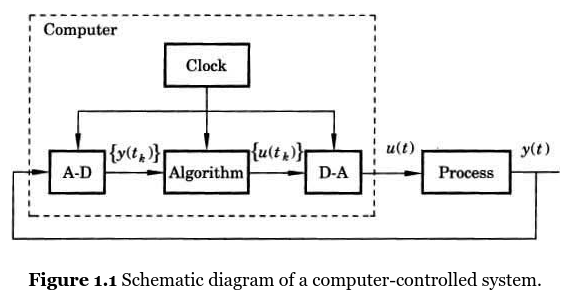
\includegraphics[width=0.7\linewidth]{../../figures/fig1-1-schematic.png}
\end{center}
{\footnotesize Åström \& Wittenmark \textit{Computer-controlled systems}}
\end{frame}
\begin{frame}[label={sec:orgca009df}]{Sampling a continuous-time system}
\begin{center}
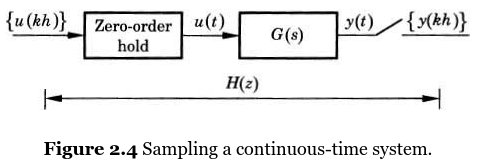
\includegraphics[width=0.6\linewidth]{../../figures/fig2-4.png}
\end{center}
{\footnotesize Åström \& Wittenmark \textit{Computer-controlled systems}}
\end{frame}
\section{Zero-order hold, or step-invariant sampling preview}
\label{sec:org9414dd4}
\begin{frame}[label={sec:org47398e9}]{Step-invariant sampling}
\begin{center}
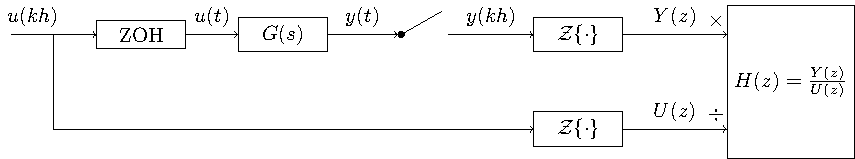
\includegraphics[width=0.99\linewidth]{../../figures/invariant-sampling.pdf}
\end{center}
\[ u(kh) = \begin{cases} 1, & k \ge 0\\0, & k<0 \end{cases} \]

\begin{tcolorbox}
\[ H(z) = \frac{z-1}{z} \ztrf{\mathcal{L}^{-1}\{ \frac{G(s)}{s} \}} \]
\end{tcolorbox}
\end{frame}

\begin{frame}[label={sec:orgab84322}]{Example: DC motor with delay}
\begin{center}
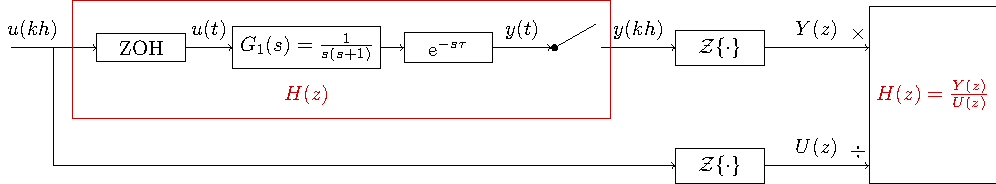
\includegraphics[width=0.89\linewidth]{../../figures/invariant-sampling-dcmotor.pdf}
\end{center}
\[ G(s) = G_1(s)\mathrm{e}^{-s\tau} = \frac{\mathrm{e}^{-s\tau}}{s(s+1)}\]

\begin{enumerate}
\item \alert{Step-response without delay} \[ \frac{G(s)}{s} = \frac{1}{s^2(s+1)} = -\frac{1}{s} + \frac{1}{s^2} + \frac{1}{s+1} \]
\[ y_1(t) = \mathcal{L}^{-1} \{-\frac{1}{s} + \frac{1}{s^2} + \frac{1}{s+1}\} = u_H(t)\big(t-1+\mathrm{e}^{-t}\big).\]
\item \alert{Step-reponse with delay} \(y(t) = y_1(t-\tau) =  -u_H(t-\tau) + u_H(t-\tau)(t-\tau) + u_H(t-\tau)\mathrm{e}^{-(t-\tau)}\big)\)
\end{enumerate}
\end{frame}

\begin{frame}[label={sec:orgb5b9ccc}]{Example: DC motor with delay}
Assuming \(\tau = nh\)
\[ \ztrf{f(kh-nh)} = z^{-n}\ztrf{f(kh)}.\]
\begin{enumerate}
\setcounter{enumi}{2}
\item \alert{Z-transform of the sampled response w/o delay} 
Usando las transformadas
\begin{align*}
u_H(kh) \quad &\overset{\mathcal{Z}}{\longleftrightarrow} \quad \frac{z}{z-1}\\
u_H(kh)kh \quad &\overset{\mathcal{Z}}{\longleftrightarrow} \quad \frac{zh}{(z-1)^2}\\
u_H(kh)\mathrm{e}^{-a(kh)} \quad &\overset{\mathcal{Z}}{\longleftrightarrow} \quad \frac{z}{z-\mathrm{e}^{-ah}}
\end{align*}

\pause
\[Y_1(z) = -\frac{z}{z-1} + \frac{zh}{(z-1)^2} + \frac{z}{z-\mathrm{e}^{-h}}\]
\end{enumerate}
\end{frame}

\begin{frame}[label={sec:org4d66e20}]{Example: DC motor with delay}
\begin{enumerate}
\setcounter{enumi}{3}
\item \alert{Z-transform of the delayed response}
\[ Y(z) = z^{-n} \left(-\frac{z}{z-1} + \frac{zh}{(z-1)^2} + \frac{z}{z-\mathrm{e}^{-h}}\right)\]
\item \alert{Dividing with the z-transform of the step} 
\begin{align*}
H(z) &= \frac{Y(z)}{U(z)} = \frac{z-1}{z} z^{-n} \left(-\frac{z}{z-1} + \frac{zh}{(z-1)^2} + \frac{z}{z-\mathrm{e}^{-h}}\right)\\
&= z^{-n} \left( -1 + \frac{h}{z-1} + \frac{z-1}{z-\mathrm{e}^{-h}} \right)\\
&= \frac{ z\big( h-1+\mathrm{e}^{-h}\big) - \big(\mathrm{e}^{-h}(1+h) - 1\big)}{z^n(z-1)(z-\mathrm{e}^{-h})}
\end{align*}
\end{enumerate}
\end{frame}

\begin{frame}[label={sec:org51c6fe6}]{Example: DC motor with delay}
\[ G(s) = \frac{\mathrm{e}^{-s(nh)}}{s(s+1)} \quad \longrightarrow \quad
   H(z) = \frac{ z\big( h-1+\mathrm{e}^{-h}\big) - \big(\mathrm{e}^{-h}(1+h) - 1\big)}{z^n(z-1)(z-\mathrm{e}^{-h})}\]
\alert{Activity} Determine the zero and the poles for the case \(n=1\) y \(h=0.2\), and mark them in the corresponding diagrams (mark zero with  \tikz \draw (1ex,.7ex) circle (.8ex); and poles with \(\times\)).
\begin{columns}
\begin{column}{0.4\columnwidth}
\begin{tikzpicture}
\node[red] at (-1.5,2) {\Large $s$-plane};
\draw[->] (-2,0) -- (1,0); 
\draw[->] (0,-2) -- (0,2);
\end{tikzpicture}
\end{column}


\begin{column}{0.6\columnwidth}
\begin{tikzpicture}
\node {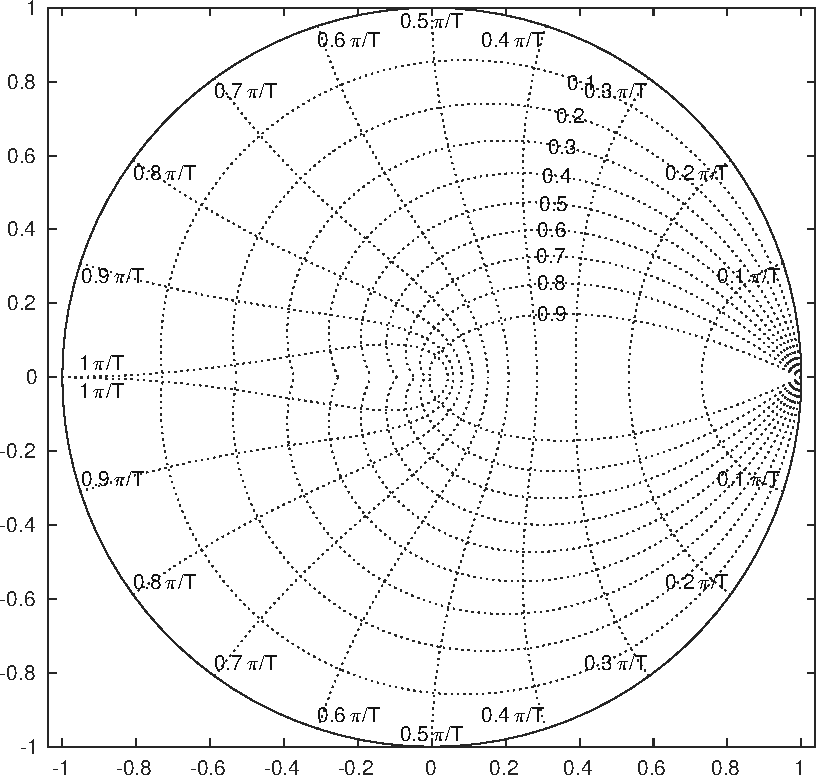
\includegraphics[height=0.6\textheight]{../../figures/zgrid-crop}};
\node[red] at (2.5,2.2) {\Large $z$-plane};
\end{tikzpicture}
\end{column}
\end{columns}
\end{frame}

\section{The map from the s-plane to the z-plane}
\label{sec:org787e461}
\begin{frame}[label={sec:org59c7520}]{Mapping from the \(s\)-plane to the \(z\)-plane}
\begin{tcolorbox}
\[ z = \mathrm{e}^{sh} \qquad \Leftrightarrow \qquad  s = \frac{1}{h} \ln z\]
\end{tcolorbox}

\alert{Important example} The left half-plane of the \(s\)-plane : \(s = a + i\omega, \; a < 0, \; -\infty < \omega < \infty\)
\[ z = \mathrm{e}^{sh} = \mathrm{e}^{(a + i\omega)h} = \mathrm{e}^{ah} \mathrm{e}^{i\omega h}, \quad |z| = |\mathrm{e}^{ah}|\, |\mathrm{e}^{i\omega h}| = |\mathrm{e}^{ah}| < 1, \; a < 0\]
\end{frame}
\end{document}